\chapter{Análisis del problema} \label{chap:Analisis}

\section{Introducción}
Como vimos en el capítulo anterior, el área de \emph{mobile forensics} no cuenta con procedimientos tan bien definidos a la hora de realizar una extracción de datos como se cuenta en el caso de los PC.

Por la naturaleza del ecosistema Android, los dispositivos móviles son diseñados por una gran diversidad de fabricantes. Los mismos poseen cierto grado de libertad a la hora de implementar las funcionalidades que ofrecen a través del sistema operativo Android. Esto lleva a que frecuentemente nos encontremos con componentes que son implementados de diferente forma por distintos fabricantes. Por ejemplo, un fabricante puede optar por utilizar un filesystem distinto al de referencia (EXT4) para la partición que almacena los datos del usuario \cite{adrdstrg}. Estas diferencias, que para el usuario final del dispositivo no suelen ser perceptibles, tienen un impacto considerable en la forma de extraer los datos.

Vemos entonces que a pesar de que los tipos de datos que podemos extraer de los dispositivos Android son en esencia los mismos, la forma en la cual debemos realizar su extracción muy a menudo varía dependiendo de variables como son el fabricante del dispositivo y la versión del sistema operativo Android.

La dependencia en la implementación por parte del fabricante se hace mayor si consideramos realizar extracciones físicas. En el caso de extracciones lógicas, tenemos una menor dependencia con la implementación del fabricante por el simple hecho de contar con las abstracciones y convenciones que establece la plataforma Android, pero aún así existen muchos aspectos en los cuales seguimos dependiendo de la implementación del fabricante también a este nivel. A modo de ejemplo, un caso habitual es el esquema de la base de datos utilizada para almacenar los mensajes de texto. Dicho esquema suele variar dependiendo el fabricante e incluso entre carriers \cite{delsms}.

Por otro lado, también dependemos de la versión de Android que posee el dispositivo. A menudo se producen cambios en la plataforma que provocan que debamos modificar la forma en la que extraemos los datos ya sea porque cambia la forma en que se acceden o presentan los datos. Por ejemplo, en la versión 4.1 de Android se restingió el acceso a logs de aplicaciones. Previo a esto, aplicaciones de terceros tenían la capacidad de solicitar el permiso \emph{READ\_LOGS} con el cual podían acceder a los logs generados por las demás aplicaciones \cite{logaccss}.

Por lo tanto, vemos que contar con un nivel de abstracción que permita concentrarnos en qué datos deseamos extraer, sin tener que estar considerando cómo extraerlos de cada dispositivo en particular, sería de gran utilidad para poder desarrollar herramientas y procesos forenses que escalen ante la gran variedad del ecosistema Android.

Asimismo, tener este nivel de abstracción no sólo resultaría útil para uniformizar el proceso de extracción de datos a través de diversos dispositivos y versiones de Android, sino que también podría facilitar la forma en que especificamos los datos que deseamos extraer. De esta forma, sería interesante poder realizar extracciones especificando únicamente el tipo y la fuente de los datos a obtener.

Por último, vemos que este nivel de abstracción también nos brinda la oportunidad de poder \enquote*{empaquetar} las técnicas de extracción de datos de una forma uniforme. Esto permite que luego de desarrolladas puedan ser compartidas y reutilizadas por otros. Este aspecto resulta vital para crear un ambiente de desarrollo colaborativo el cual permita soportar una porción considerable del ecosistema Android.

Las consideraciones arriba descritas respaldan nuestra convicción de la necesidad de contar con una herramienta que asista en la extracción de datos de dispositivos móviles Android podría favorecer sustancialmente el trabajo del investigador forense. En la siguiente sección describiremos los problemas que apuntamos resolver mediante la creación de la misma.

\section{Objetivos planteados}
El objetivo principal de la herramienta propuesta es \textbf{facilitar la extracción de datos} de dispositivos móviles Android. Para esto, la herramienta deberá realizar una fuerte separación entre cómo el usuario expresa lo que desea extraer y cómo se lleva a cabo la extracción. Esta separación permite a los usuarios concentrarse en qué datos extraer y no en cómo debe implementar el procedimiento de extracción. De esta forma, evitamos que los usuarios requieran contar con amplio conocimiento técnico para utilizar la herramienta, lo cual permite que la misma sea utilizada por un espectro más amplio de investigadores forenses.

Como vimos, una de las características fundamentales del ecosistema Android es su diversidad. Esto hace que sea importante abordar el desafío de extraer datos de forma escalable desde la concepción de la herramienta. Para esto, la misma deberá contar con una arquitectura que \textbf{facilite su extensibilidad} con el fin de poder soportar rápidamente nuevas formas de extraer datos. Esta es una necesidad clave ante la permanente evolución de Android y su ecosistema de dispositivos.

Finalmente, otro aspecto clave a resolver es el hecho de que hoy en día las herramientas forenses cuentan con escasa interoperabilidad entre ellas. Independientemente de los motivos comerciales o políticos que haya detrás de este hecho, consideramos que uno de los aspectos más importantes para que la herramienta resulte útil en la práctica radica en \textbf{facilitar la manipulación de los datos extraídos}. Por lo tanto, la herramienta debe brindar sus salidas en un formato que facilite la consumición de las mismas por parte de herramientas de análisis forense. Por esta razón, creemos razonable buscar la adopción de lenguajes o formatos estándares en el área para expresar las salidas de la herramienta.

\section{Enfoque inicial}
Para cumplir con los objetivos propuestos nos planteamos cómo debería ser la interacción que proporciona la herramienta y las operaciones que la misma brinda. A continuación analizaremos cómo llegamos a decidir varios de los aspectos claves que luego veremos reflejados en el funcionamiento de la herramienta.

Si consideramos el comportamiento más simple que uno esperaría de una herramienta de este tipo, seguramente sería el de contar con un conjunto de operaciones de extracción definidas y ser capaz de extraer exactamente los datos que deseamos con una única operación. Esto nos lleva a considerar cómo dividiríamos el dominio de operaciones de extracción con el que debemos contar. Al considerar las variables descritas anteriormente, surgen naturalmente dos enfoques que coinciden con casos de uso habituales para un investigador:

\begin{itemize}
\item Por un lado, nos puede interesar realizar extracciones según la \textbf{fuente de datos}. Por ejemplo, un investigador podría desear obtener todos los datos relevantes de la aplicación Facebook.
\item Por otro lado, también puede ser interesante poder realizar extracciones según su \textbf{tipo de datos}. Por ejemplo, un investigador podría desear obtener todas las imágenes del dispositivo (ya sean estas de Facebook, WhatsApp, la cámara, etc).
\end{itemize}

En vez de tener que decidir por uno de los dos enfoques, vimos que sería muy interesante intentar satisfacer ambas necesidades. Para esto, nos dimos cuenta que esto es posible si consideramos operaciones de extracción concisas que luego puedan ser combinadas para obtener los datos deseados. En vez de intentar dividir el conjunto de operaciones utilizando únicamente una de estas variables (esto es, en operaciones dedicadas a extraer datos o bien según su tipo de dato, o bien según su fuente de datos), lo dividiríamos según ambas.

Finalmente, vemos que de esta forma la herramienta contaría con operaciones más granulares, pero al combinarlas nos permitirían extraer con precisión los datos deseados. Por lo tanto, logramos así que la herramienta tenga una mayor flexibilidad al abarcar ambos casos de uso. De hecho, este enfoque permite que la misma tenga una mayor capacidad de expresión, pudiendo llegar a ser bien específicos en los datos que deseamos extraer al fijar tanto tipo de dato como fuente de datos. Por ejemplo, nos permitiría expresar tanto el deseo de extraer únicamente las imágenes de Facebook, como el de obtener todos los mensajes de texto del dispositivo (sin importar si estos provienen de Hangouts ó WhatsApp).

En resumen, el enfoque que tomamos para concebir una operación nos ofrece lo siguiente:

\begin{itemize}
\item \textbf{Expresividad}: Permite tener un nivel de precisión muy interesante en los datos que deseamos extraer.
\item \textbf{Flexibilidad}: Permite cubrir distintos casos de uso de forma simple.
\item \textbf{Extensibilidad}: Posibilita un diseño que permite ser extendido para soportar nuevas propiedades de operaciones.
\end{itemize}

\section{Conceptos fundamentales}
\label{conceptos_fundamentales}
Empecemos por detallar mejor dos de los conceptos claves que mencionamos. Estos son: fuente de dato y tipo de dato. En base a los mismos es que determinamos la granularidad que tendrán las operaciones, como vimos en el enfoque recién planteado.

La información que solemos encontrar en los dispositivos móviles puede provenir de diversas \textbf{fuentes de datos}. A su vez, resulta interesante observar que hay conjuntos de fuentes de datos para los cuales el mecanismo para obtener datos de las mismas es el mismo. En estos casos, decimos que dichas fuentes son del mismo \textbf{tipo de fuente de dato}.

Por otro lado, las diversas piezas de información que podemos encontrar en los dispositivos poseen una semántica diferente para el usuario dependiendo del concepto que representan. Las piezas de información que representan un mismo concepto las asociamos a un \textbf{tipo de dato}.

En el enfoque planteado, vimos que cada operación realiza un trabajo conciso. De esta forma, una \textbf{operación de extracción} extrae un único tipo de dato, de una única fuente de datos y para determinado rango de versiones y modelos de dispositivos Android.

Ahora que hemos visto lo que hace una operación de extracción, resulta importante que precisemos el término utilizado para referirnos a ella. Si bien la herramienta fue enfocada desde su concepción a la extracción de datos, esta no es exclusivamente la única tarea que realiza una operación.

Además de extraer los datos originales, deseamos encontrar únicamente los de cierto tipo de dato y luego representar la información encontrada sobre los mismos en cierto lenguaje. Estas tareas no caen exclusivamente en la etapa que se conoce como extracción en la mayoría de los modelos de proceso forense. Tomemos para esto como referencia el modelo propuesto y utilizado por el Departamento de Justicia de EEUU \cite{eleccrime} y veamos las tres etapas del proceso forense en que participa una operación:

\begin{itemize}
\item \textbf{Extracción}, dado que se encarga de obtener datos de una fuente de datos del dispositivo.
\item \textbf{Examinación}, dado que identifica y presenta datos hallados (correspondientes con el tipo de dato de la operación), en un nivel de abstracción mayor al de los datos obtenidos originalmente.
\item \textbf{Presentación}, dado que los datos hallados serán expresados en cierto lenguaje estándar.
\end{itemize}

\section{Requerimientos}
A continuación describiremos los requerimientos con los cuales consideramos que debe cumplir la herramienta para lograr los objetivos planteados.

\subsection*{A. Funcionalidades claves}
La herramienta debe proveer al usuario un conjunto de operaciones que faciliten la extracción de datos de dispositivos móviles Android. Para esto, la misma debe brindar las siguientes funcionalidades claves:

\subsubsection*{A1. Operaciones atómicas} \label{reqA1}
Las operaciones deben contar con un alto nivel de granularidad. De esta forma, una operación debe extraer un único tipo de dato, de una fuente de datos determinada, soportando un determinado conjunto de dispositivos y versiones de Android.

\subsubsection*{A2. Consulta de operaciones} \label{reqA2}
La herramienta debe contar con la posibilidad de consultar (y filtrar) por las operaciones disponibles. De esta forma, el usuario puede descubrir las mismas y sus características.

\subsubsection*{A3. Ejecución de operaciones} \label{reqA3}
La herramienta debe permitir ejecutar una serie de operaciones en un único paso. Esto permite al usuario combinar operaciones y, debido al alto nivel de granularidad que poseen las mismas, tener la capacidad de extraer con gran precisión los datos deseados.

\subsubsection*{A4. Modos de ejecución de la herramienta} \label{reqA4}
La herramienta debe contar con dos modos de ejecución:
\begin{itemize}
\item Un \textbf{modo interactivo}, en el cual el usuario pueda realizar consultas sobre las operaciones disponibles filtrando por los parámetros de las mismas y luego ejecutar las operaciones deseadas.
\item Un \textbf{modo batch}, en el cual el usuario ya conoce las operaciones que desea utilizar y únicamente especifica cuáles ejecutar.
\end{itemize}

\subsection*{B. Extensibilidad} \label{reqB}
La herramienta debe proveer mecanismos que permitan extender fácilmente los siguientes tres puntos:
\begin{enumerate}[topsep=0pt, parsep=0pt, partopsep=0pt]
\item Tipos de datos
\item Tipos de fuente de datos
\item Operaciones
\end{enumerate}

\subsection*{C. Acceso de datos} \label{reqC}
La herramienta debe ser capaz de abstraer la forma en que accede a los datos. De esta forma, posibilita su interoperación tanto con la diversidad de dispositivos reales que hay como con emuladores, y además permite la extensibilidad de la herramienta para soportar otros dominios de datos.

\subsection*{D. Salida de datos}
\subsubsection*{D1. Lenguaje estándar} \label{reqD1}
La herramienta debe hacer uso de un lenguaje estándar para expresar sus salidas de datos, con el fin de que para otras herramientas sea sencillo consumir los datos producidos.

\subsubsection*{D2. Lenguaje extensible} \label{reqD2}
Además, el lenguaje utilizado para representar los datos de salida debe ser extensible, dado que es necesario que el mismo sea capaz de representar información de nuevos tipos de datos.

\section{Casos de uso}
Vistos los requerimientos, ahora vamos a considerar los casos de uso necesarios para satisfacer a los mismos.

Comencemos por describir al usuario el cual apuntamos que haga uso de nuestra herramienta. El mismo lo concebimos como un investigador forense, el cual no necesariamente cuenta con conocimiento técnico de cómo se implementa cada operación.

Deseamos que este usuario pueda hacer uso de la herramienta principalmente de dos posibles formas:

\begin{enumerate}[topsep=0pt, parsep=0pt, partopsep=0pt]
\item Manual, esto es, interactuando directamente con la herramienta con el fin de obtener los datos que desea de un cierto dispositivo.
\item Automática, con el fin de permitirle automatizar tareas de obtención de datos o facilitar la integración de la herramienta con otras herramientas utilizadas por el usuario.
\end{enumerate}

Para estos dos casos de uso es que la herramienta posee dos modos distintos de ejecución, interactivo y batch respectivamente, que son establecidos en \hyperref[reqA4]{(Req. A4)}.

En tanto, en \hyperref[reqB]{(Req. B)} se expresa la capacidad de extensibilidad que debe tener la herramienta. Veremos cómo el sistema tiene dicha capacidad mediante dos casos de uso que permiten agregar y eliminar operaciones del sistema. Estos se centran en el punto de extensión que es de mayor interés para la herramienta. También consideraremos los otros dos puntos de extensión, que auspician de soporte al anterior, en el caso de agregar una operación y que la misma haga uso de un tipo de dato o tipo de fuente de dato nueva al sistema.

Finalmente, el usuario tiene a su disposición el siguiente conjunto de comandos para interactuar con el sistema:
\newline

\footnotesize
    \renewcommand*{\arraystretch}{1.4}
    \begin{longtable}{ | >{\bfseries}m{4.8cm} | >{\itshape}m{8.2cm} | >{\itshape}c |}
    \hline
    \BlackCell{Comando} & \BlackCell{Descripción} \\ \hline \hline
    set\_device\_info & Permite especificar la información del dispositivo en el modo de ejecución interactivo. Esto hace posible que podemos omitir dicha información de los comandos \texttt{list} y \texttt{execute} posteriores. \\ \hline
    
    list & Lista las operaciones disponibles del sistema. Es de especial valor su uso en el modo interactivo, ya que permite al usuario descubrir las operaciones y sus características. \\ \hline
    
    execute & Permite ejecutar un conjunto de operaciones tanto en modo interactivo como en modo batch. \\ \hline
    
    add\_ext & Permite añadir una nueva extensión al sistema, ya sea operación, tipo de dato o tipo de fuente de datos. \\ \hline
    
    rm\_ext & Permite eliminar una extensión del sistema. En el caso de tipo de datos y tipo de fuentes de datos, la eliminación de la extensión se llevará a cabo únicamente en caso que la misma no esté siendo utilizada por ninguna operación. Si deseamos eliminarla, primero será necesario eliminar explícitamente las operaciones que hacen uso de la misma. \\ \hline
    \caption {Comandos disponibles de la herramienta}
    \label{tab:objetos}
    \end{longtable}
    \normalsize

\subsection{Ejecución de operaciones en modo interactivo}

\subsubsection*{Flujo principal}
\begin{enumerate}
\item El usuario ejecuta la herramienta sin ningún parámetro adicional.
\item El sistema inicia una sesión de ejecución interactiva.
\item El usuario ejecuta el comando \texttt{list} indicando el tipo de datos, la fuente de datos (y la información del dispositivo en caso de no haber utilizado el comando \texttt{set\_device\_info}).
\item El sistema retorna la información de todas las operaciones que cumplen con los valores indicados. Para cada operación se muestra:
    \begin{itemize}
    \item Nombre de la operación.
    \item Tipo de datos que examina.
    \item Fuente de datos utilizada para extraer los datos.
    \item Modelos de dispositivos soportados
    \item Versiones de Android soportadas.
    \end{itemize}
\item El usuario ejecuta el comando \texttt{execute} indicando los nombres de las operaciones que desea ejecutar (y la información del dispositivo en caso de no haber utilizado el comando \texttt{set\_device\_info}).
\item Para cada operación ejecutada:
    \begin{itemize}
    \item Si completó exitosamente, el sistema indica la ruta al directorio en donde fue almacenada la información obtenida.
    \item Sí falló, el sistema indica la causa.
    \end{itemize}
\item El usuario no desea realizar más extracciones.
\item Fin del caso de uso.
\end{enumerate}

\subsubsection*{Flujos alternativos}

\begin{itemize}
\item 3A.
    \begin{enumerate}
    \item El usuario ejecuta el comando \texttt{set\_device\_info} indicando la información del dispositivo.
    \item El sistema guarda la información del dispositivo. Esta información será tenida en cuenta por los comandos \texttt{list} y \texttt{execute}.
    \item Retorna al paso 3 del flujo principal.
    \end{enumerate}
\end{itemize}

\begin{itemize}
\item 5A.
    \begin{enumerate}
    \item El usuario ejecuta el comando \texttt{execute} indicando los nombres de las operaciones que desea utilizar, pero no indica la información sobre el dispositivo.
    \item El sistema retorna un mensaje de error indicando que es necesario conocer la información del dispositivo.
    \item Se retorna al paso 5 del flujo principal.
    \end{enumerate}
\end{itemize}

\begin{itemize}
\item 7A. El usuario desea realizar otra extracción.
    \begin{enumerate}
    \item Se retorna al paso 3 del flujo principal.
    \end{enumerate}
\end{itemize}

\subsection{Ejecución de operaciones en modo batch}
La diferencia más importante entre este modo de ejecución de operaciones y el modo previamente explicado consiste en que en este modo el usuario ya sabe cuales son las operaciones que desea ejecutar. Por lo tanto, no necesita de un modo interactivo en donde realizar consultas previo a ejecutar las operaciones.

\subsubsection*{Flujo principal}
\begin{enumerate}
\item El usuario ejecuta la herramienta pasándole como parámetro el comando \texttt{execute} seguido de los nombres de las operaciones que desea ejecutar y la información sobre el dispositivo.
\item Para cada operación ejecutada:
    \begin{itemize}
    \item Si completó exitosamente, el sistema indica la ruta al directorio en donde fue almacenada la información obtenida.
    \item Sí falló, el sistema indica la causa.
    \end{itemize}
\item Fin del caso de uso.
\end{enumerate}

\subsubsection*{Flujos alternativos}
\begin{itemize}
\item 1A.
    \begin{enumerate}
    \item El usuario ejecuta la herramienta pasándole como parámetro \texttt{execute} sin indicar los nombres de las operaciones a ejecutar y/o la información sobre el dispositivo.
    \item El sistema retorna un mensaje de error indicando los datos omitidos.
    \item Fin del caso de uso.
    \end{enumerate}
\end{itemize}

\subsection{Adición de una extensión}

\subsubsection*{Flujo principal}
\begin{enumerate}
\item El usuario ejecuta (ya sea en modo batch ó interactivo) el comando \texttt{add\_ext} pasándole como parámetros el tipo de extensión (operación, tipo de dato o tipo de fuente de datos) que desea agregar y la ruta a la definición de la nueva extensión.
\item El sistema valida la definición de la nueva extensión, la agrega y le indica al usuario que la misma fue agregada exitosamente.
\item Fin del caso de uso.
\end{enumerate}

\subsubsection*{Flujos alternativos}
\begin{itemize}
\item 1A.
    \begin{enumerate}
    \item El usuario desea agregar una operación y la misma utiliza un tipo de dato o un tipo de fuente de datos que no existe en el sistema.
    \item El sistema le indica al usuario que la definición de la operación hace uso de una extensión que no se encuentra en el sistema y la misma debe ser agregada previamente para poder añadir esta operación.
    \item Fin del caso de uso.
    \end{enumerate}
    
\item 2A. / 1A.2A
    \begin{enumerate}
    \item El sistema determina que la definición de la extensión recibida es inválida.
    \item El sistema retorna un mensaje de error indicando los campos inválidos de la definición.
    \item Fin del caso de uso.
    \end{enumerate}
\end{itemize}

\subsection{Eliminación de una extensión}

\subsubsection*{Flujo principal}
\begin{enumerate}
\item El usuario ejecuta (ya sea en modo batch ó interactivo) el comando \texttt{rm\_ext} pasándole como parámetros el tipo de la extensión que desea eliminar y su nombre.
\item El sistema elimina la extensión e informa al usuario de ello.
\item Fin del caso de uso.
\end{enumerate}

\subsubsection*{Flujo alternativo}
\begin{itemize}
\item 1A.
    \begin{enumerate}
    \item El usuario ejecuta el comando \texttt{rm\_ext} sin indicar el tipo y/o nombre de la extensión que desea eliminar.
    \item El sistema retorna un mensaje de error haciendo referencia a los parámetros faltantes.
    \item Fin del caso de uso.
    \end{enumerate}
\end{itemize}

\subsection{Diagrama de casos de uso}
De forma de resumir la interacción entre el usuario y el sistema, en la figura \ref{diagramaCasosDeUso} se muestran los casos de uso en base a dos roles:

\begin{itemize}
\item El primero de ellos trata del rol \emph{usuario}, el cual permite utilizar al sistema tanto en modo interactivo como en modo batch.
\item El segundo trata del rol \emph{administrador}, el cual permite configurar la herramienta agregando y removiendo extensiones de la misma.
\end{itemize}

\begin{figure}[H]
    \begin{center}
        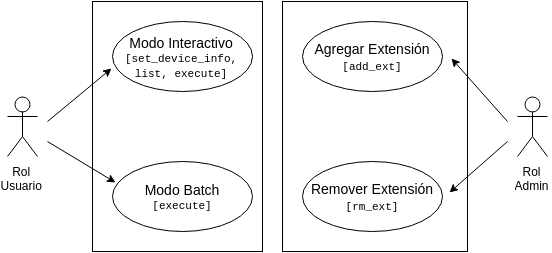
\includegraphics[width=\textwidth]{figures/diagrama_casos_de_uso}
        \caption{Diagrama de casos de uso}
        \label{diagramaCasosDeUso}
    \end{center}
\end{figure}

\section{Definición del alcance}
En base a los requerimientos establecidos, veremos a continuación varios aspectos que merecen ser mencionados con el fin de ayudar a delimitar con claridad el alcance del proyecto.

\subsection*{A. Funcionalidades claves} \label{FuncionalidadesClavesAlcance}
Como vimos en el requerimiento \hyperref[reqA1]{A1}, la herramienta contará con un conjunto de operaciones las cuales realizan la extracción, examinación y presentación de los datos encontrados. A través de dichas operaciones, la herramienta manejará:

\begin{itemize}
\item \textbf{Datos extraídos de dispositivos móviles} de carácter lógico y orientados a aquellos producidos por los usuarios de los mismos (esto es, no nos enfocaremos en examinar datos producidos por malware, por ejemplo). De todas formas, la arquitectura de la herramienta será diseñada de manera de facilitar la incorporación de otros dominios de datos.
\item \textbf{Datos sobre el proceso de extracción}. En primer lugar, será de interés conocer la relación entre los datos que fueron originalmente extraídos del dispositivo y la información examinada (esto es, dada una pieza de información examinada deseamos conocer de qué fuente, por ejemplo de qué archivo, se extrajo dicha información). En segundo lugar, será de interés contar con información sobre quién, cuándo, cómo y dónde se utilizó la herramienta para extraer los datos. Para esto, buscaremos incluir información sobre los colaboradores, fecha y hora de la extracción y datos del ambiente utilizado.
\end{itemize}

En cuanto al mecanismo de consulta de operaciones descrito en \hyperref[reqA2]{A2}, el prototipo de la herramienta contará con capacidades básicas de filtrado. Seguramente pueda ser útil contar con opciones más avanzadas de filtrado (como expresiones lógicas) con el fin de facilitar el uso de la herramienta, pero consideramos que esto sería más adecuado hacerlo en una segunda iteración.

\subsection*{B. Extensibilidad} \label{ExtensibilidadAlcance}
\subsubsection*{Tipos de fuentes de datos}
El prototipo de la herramienta estará enfocado en la extracción de datos de aplicaciones. Para esto, contaremos con un tipo de fuente de datos que llamaremos \emph{Application} y el cual permitirá tomar como fuente de datos aquellos datos pertenecientes a una aplicación instalada en el dispositivo.

Cabe destacar que, de todas formas, será fundamental que la herramienta tenga un diseño extensible que le permita soportar otros tipos de fuentes de datos como establecimos en \hyperref[reqB]{(Req. B)}. Por esta razón, vemos que como contrapartida a datos de aplicaciones, sería interesante desarrollar (en una futura iteración de la herramienta) la extracción de datos del sistema operativo. Esta posibilidad se expresa en más detalle en la sección \ref{OtrosTiposDeExtractors}.

\subsubsection*{Tipos de datos}
El prototipo de la herramienta por defecto contará con un conjunto básico de tipos de datos correspondientes a los diversos objetos predefinidos por el lenguaje.

A modo de ejemplo, veamos a continuación el estilo de tipos de datos que pretenderemos poder representar mediante el mismo, ya sea utilizando objetos predefinidos o extendiendo el lenguaje.

Para el dominio de \emph{datos de aplicaciones}, desearíamos poder representar:
\begin{itemize}
\item Mensajes de texto (SMS, MMS)
\item Mensajes de chat (Hangouts, WhatsApp, Facebook)
\item Mensajes de correo (Android default email app, GMail)
\item Contactos (Android default agenda app, Facebook, GMail)
\item Registro de llamadas
\item Eventos de calendario (Google Calendar)
\item Archivos (Locales, GDrive, Dropbox)
\item Información de ubicación (GPS, geo-fencing)
\item Historial de navegación (Chrome, Firefox)
\end{itemize}

Para el dominio de \emph{datos del sistema}, desearíamos poder representar:
\begin{itemize}
\item Datos de telefonía (ICCID, IMEI, MEID)
\item Información de red (Dirección MAC de Wi Fi, Bluetooth)
\item Información del dispositivo (Modelo, marca)
\item Procesos corriendo
\item Conexiones activas
\end{itemize}

En el primer grupo vemos ejemplos de tipos de datos que podemos obtener de fuentes de datos del tipo de \emph{Application} como con los que nos enfocaremos. En el segundo, vemos ejemplos de datos relevantes al sistema, que si bien no los consideraremos directamente, ya mencionamos que es importante que el lenguaje pueda representarlos para que luego sea posible extender la herramienta y soportar su uso.

\subsubsection*{Operaciones}
El prototipo de la herramienta contará con un conjunto de operaciones por defecto, las cuales serán desarrolladas como parte del caso de estudio.

\subsection*{C. Acceso de datos}
Como vimos, este requerimiento busca abstraer la forma utilizada por la herramienta para acceder a los datos con el fin de poder interoperar con múltiples tipos de dispositivos (incluso con emuladores).

En este sentido, el protocolo ADB (Android Debug Bridge) y sus herramientas nos proveen la abstracción necesaria que precisamos para cumplir con el requerimiento \hyperref[reqC]{(Req. C)}. El mismo nos posibilita el intercambio de datos y ejecución de comandos de forma transparente, tanto en dispositivos físicos como en emuladores.

Para el ambiente de desarrollo del prototipo, utilizaremos un emulador Android por la flexibilidad, facilidad y control que esto nos brinda. En particular:

\begin{itemize}
\item Nos da la posibilidad de crear imágenes específicas del estado de un dispositivo.
\item Evitamos preocuparnos por fallas o pérdida de datos de un dispositivo real.
\item Podemos contar con acceso root al dispositivo de manera muy sencilla, lo cual nos permitirá acceder a todos los datos del mismo.
\end{itemize}

De todas formas, la herramienta será diseñada para soportar tanto dispositivos reales como virtuales (emuladores). El hecho de contar con una interfaz de acceso a los dispositivos como es \emph{adb} y un emulador que imita al hardware de un dispositivo real hace que esta transición, en teoría, no deba requerir esfuerzo adicional.

\subsection*{D. Salida de datos}
Debido al funcionamiento que comprende una operación, vemos que la herramienta deberá contar con los siguientes tipos de salida de datos:

\begin{itemize}
\item \textbf{Datos extraídos}, para expresar los datos que fueron obtenidos del dispositivo en su forma original.
\item \textbf{Datos examinados}, para expresar los datos encontrados a partir de los anteriores.
\item \textbf{Datos del proceso de extracción}, para expresar información acerca de los colaboradores que obtuvieron los datos examinados, el ambiente que utilizaron y los archivos de los cuales fue obtenida la información de los mismos.
\end{itemize}

De manera de cumplir con los requerimientos [Req. D1] y [Req. D2], utilizaremos el lenguaje CybOX para representar a las salidas de datos examinados y del proceso. El lenguaje ya fue analizado extensamente en la sección \ref{estadoDelArte:CybOX} en donde vimos cómo el mismo cumple con los requerimientos mencionados (esto es, es estándar y extensible). Además, vimos como el lenguaje posibilita la representación de los tipos de datos mencionados en los puntos \hyperref[FuncionalidadesClavesAlcance]{A} y \hyperref[ExtensibilidadAlcance]{B} de esta sección de Definición del Alcance.
